%! Date = 28/03/2023

% Preamble
\documentclass[a4paper,12pt]{article}

\usepackage[utf8]{inputenc}
\usepackage[T1]{fontenc}
\usepackage{lmodern}
\usepackage[english]{babel}
\usepackage{graphicx}
\usepackage[style=authoryear]{biblatex}
\usepackage{url}
\usepackage{hyperref}
\usepackage{booktabs}
\usepackage{tabularx}
\usepackage{pdflscape}
\usepackage{placeins}
\usepackage{geometry}
\geometry{
    a4paper,
    total={170mm,257mm},
    left=30mm,
    right=30mm,
    top=25mm,
    bottom=25mm,
}
\addbibresource{references.bib}

\begin{document}
    \begin{titlepage}
        \begin{center}
        {\huge\bfseries Suitability of an Internal Developer Portal to Support the Daily Work of BizDevOps Engineers\par}
            \vspace{2cm}

            {\scshape\large Certificate work in the \par}
            {\scshape\large CAS Digital Product Lead \par}
            \vspace{1cm}

            {\scshape\large HWZ University of Applied Sciences \par}
            {\scshape\large for Business Administration Zurich \par}
            \vspace{4cm}

            {\normalsize submitted to\par}
            \vspace{0.5cm}

            {\large Ralph Hutter\par}
            \vfill
            {\normalsize submitted by\par}
            \vspace{0.5cm}
            {\large Thierry Peng\par}
            \vspace{0.5cm}
            {\normalsize Address: placeholder 68, placeholder\par}
            {\normalsize  Place, Date: placeholder, \today\par}

        \end{center}
    \end{titlepage}


    \section*{Management Summary}
    %TODO
    \pagebreak


    \tableofcontents
    \pagebreak

    \section*{Used Tools}
    In addition to the sources mentioned in the bibliography, chapter \ref{sec:bibliograhpy}, the following aids and tools have been used
    \begin{itemize}
        \item Version control with Git and GitHub, the source code for this document is at \url{https://github.com/thpeng/mas/tree/master/src/mca-dpl23-1}
        \item Deepl at (\url{https://www.deepl.com/}) to support translations.
        \item Microsoft Forms to conduct a survey (\url{https://forms.office.com}) .
        \item The document is written in \LaTeX  (\url{https://miktex.org/}) with the editor IntelliJ IDEA (\url{https://www.jetbrains.com/de-de/idea/})
    \end{itemize}

    \section*{Declaration of Honour}

    I hereby confirm that I have
    \begin{itemize}
        \item prepared the present thesis independently and without the use of sources or aids other than those indicated,
        \item identified the sources used as such, either verbatim or in terms of content,
        \item not yet submitted this work in the same or similar form to an examination board.
    \end{itemize}
    Bern, \today\newline
    \newline
    \newline
    \newline
    \begin{tabular}{@{}p{5.0cm}@{}}
        \hrulefill \\
        Thierry Peng
    \end{tabular}

    \pagebreak

    % max 15 - 20 pages beginning here


    \section{Introduction}
    \label{sec:introduction}
    SBB has an extensive and steadily growing IT landscape of applications and tools to support the digitization of its
    core business processes.
    These digitization efforts brought major changes to the SBB IT department.
    In less than ten years, the development model has changed from a pure waterfall to an agile methodology,
    cloud technologies were adopted while hardware-bound platforms were phased out, and a new internal organization,
    based on the separation of business and line management, has been introduced.\\
    Even though these changes are now taking root and leading to various positive outcomes, they still pose a challenge.
    There is a new complexity with the rapidly changing technological landscape but also due to very many old,
    business-critical legacy systems.
    In addition, regulatory pressure has increased significantly in recent years, as exemplified by the
    HCBöV\footnote{Handbuch Cybersecurity für Betriebe des öffentlichen Vekehrs}, as well as the new Data Protection Act in Switzerland - nDSG.\\
    Feedback from various employees in different roles from SBB so called ``Digitalen Zone`` indicates, that the overall
    increase in complexity has an impact on the daily work of DevOps\footnote{DevOps is a combination of the words
    Development and Operations and is a set of practices} engineers.
    The picture emerges that, although all information for the design, development and operation of
    applications is available in principle, it is maintained in very different places and forms.
    This makes the procurement of information for these activities time-consuming and requires that a DevOps
    engineer is already very familiar with the IT landscape of SBB .

    \subsection{Problem Statement and Controversy}
    \label{subsec:iproblemstatement}
    Research on the Internet about this problem, as well as guidance from vendors, indicates that there is greater momentum
    to address such issues with an Internal Developer Portal (IDP).
    The central promise of the concept of an Internal Developer Portal is that it can reduce the so-called
    ``cognitive load`` of DevOps engineers.\\
    An Internal Developer Portal aims to provide a one stop shop for information about teams, associated applications and
    their used infrastructure and resources for DevOps engineers.

    \subsection{Objective of the Certificate Work}
    \label{subsec:iobjective}
    The goal of this certificate thesis is to investigate whether and to what extent the above-mentioned problem
    can be solved by the introduction of an Internal Developer Portal.\\
    In a first step, the benefits of the concept of an internal developer platform are elaborated and placed in the
    into the general context of software development and the operation of IT systems in the SBB.\\
    In a second step, the problem of complexity and lack of integration is underpinned with a quantitative survey.\\
    The third part consists of bringing together the results of the survey and the value proposition and making a
    recommendation for action.


    \section{Value Proposition for an Internal Developer Portal}
    \label{sec:vp}
    An Internal Developer Portal is a web-based information catalogue which is tailored for the needs of
    engineers operating IT systems, developing software and other related work.\\
    Internal Developer Portal are proposed as the solution for perceived problems\parencite{backstagestory} of DevOps
    engineers while developing and operating IT Systems such as
    \begin{itemize}
        \item A lack of a central repository for reliable and tailored information
        \item A high cognitive load of engineers because of switching between multiple and very different tools while developing or operating IT Systems
        \item Increasing the developer experience by abstracting away complexity in infrastructure management
    \end{itemize}
    One potential source of information for using in the Internal Developer Portal is a so called Internal Developer Platform.

    \subsection{Internal Developer Platform}
    \label{subsec:vpplatform}
    Gartner makes a differentiation between the concept of an Internal Developer Portal and an Internal Developer Platform:
    ``Internal Developer Portals serve as the interface through which developers can discover and
    access Internal Developer Platform capabilities``\parencite{gartner} .
    An Internal Developer Platform (Platform), according to the COO Christoph C. Richter from Humanitec\parencite{richteretal} ,
    should consist at least of the following component:
    \begin{itemize}
        \item Application Configuration Management
        \item Infrastructure Orchestration
        \item Environment Management
        \item Deployment Management
        \item Role-Based Access Control
    \end{itemize}
    In some other sources, there are also additional components mentioned, e.g. Observability\parencite{xenon}.
    XENONSTACK as well as Humanitec mentioned before, are suppliers of Internal Developer Platform solutions with
    different capabilities.\\
    The capabilities and components of an Internal Developer Platforms, as listed before,  are not specific for the products
    of those two suppliers.
    In most contemporary IT operations or software development departments these components and practices are well-known
    and used widely.\\
    Taking for example the practices of Application Configuration, Environment and Deployment Management:
    Beyond the size of a very small team, it is necessary to use tooling to know where, in which version
    and with what configuration a software artifact was installed.
    The reason for this this may be to coordinate a new software rollout, test the software on a dedicated stage, fix bugs
    or develop new features and to solve incidents caused by your software.\\
    Thus, it can be argued, that the concept of an Internal Developer Platform is not unique to specific products
    or offerings, but can be used on a set of tooling and practices supporting IT operations and software development.
    This set of tooling and practices can be viewed as predecessors of Internal Developer Platforms and are usually
    distinct solutions or products.\\
    For example there is a separate Configuration Management Database to address the need of Application Configuration
    Management or there is a purpose built CI/CD\footnote{CI/CD stands for continuous
    integration and continuous deployment and is a practice in software engineering. Its main focus is to automate all steps
    between development and rolling out on production, such as quality assurance, building artifacts and installing them.}
    pipeline for addressing the need for a Deployment Management.
    These solutions are not necessarily integrated with each other and may be products from different vendors.
    It may be also the case, that these products or solutions were established before the advent of Agile Methodologies and DevOps.

    \subsection{DevOps}
    \label{subsec:devops}
    With DevOps, the traditional disciplines of IT operations and software development are much more integrated to
    to reduce friction, release features more frequently, and improve product quality\parencite{safedevops}.
    Prior to DevOps, it was common to use different tools and processes for the development and operations roles
    because these two roles were housed in different departments or teams.
    There is a fundamental conflict in rigidly separating the roles of developer and operator.
    Developers are measured by the speed to develop features and how quickly they respond to changing requirements.
    Operators, on the other hand, are measured on how many failures their systems have and how quickly those can be patched.\\
    One of the basic principles of DevOps was coined by Werner Vogels, the current CTO of Amazon;
    ``You build it, you run it``\parencite{vogels}.
    This means that the same team that develops the software is also responsible for its operation.
    With DevOps, a team takes full responsibility over the lifecycle of an application or platform.
    In combination with agile methodologies such as Scrum\footnote{Scrum is an iterative software development methodology}
    or SAFe\footnote{SAFe stands for Scaled Agile Framework and adds orchestration layers above agile (Scrum) teams for
    a better cross-team and product-centric alignment}, business-oriented individuals are also integrated into this
    cross-functional team.
    An example of a business-oriented role in a DevOps team is the product owner\parencite{safepo}.\\
    This also means that a team must have a wide range of skills and access to various tools needed for their work.
    Such tools can be used for activities such as requirements engineering, solution architecture, software development
    but also anything needed to operate the software.
    Especially the operation of the software is a tool-intensive work.
    There are tools for logging, monitoring, incident handling, alerting and other practices.
    In the event of an incident, a configuration management database or an enterprise architecture database are critical
    to find out who a particular application or resource belongs to.
    This information is important to determine the root cause of the incident and quickly resolve it.
    Although DevOps offers numerous benefits, it is quite a complexity for a team member to master all necessary tools and
    practices in an agile DevOps team.
    Here, the Integrated Developer Portal offers several suggestions to help individuals and teams with their day-to-day operations.

    \subsection{Internal Developer Portal}
    \label{subsec:vpportal}
    Manjunath Bhat from Gartner argues, that an Internal Developer Portal has three main characteristics\parencite{gartner}:
    \begin{itemize}
        \item Abstraction
        \item Developer-centric view
        \item Pluggable framework
    \end{itemize}
    The overarching goal of these features is to improve the DevOps experience by reducing the time it takes to search
    for information and interpret it correctly.
    The search task is supported by a centralized software catalog.
    Interpretation of the data is supported by an underlying logical model that describes the assets, technologies
    and their relationships between them.
    The logical model varies among implementations of the Internal Developer Portal, but there are some common elements.

    \subsubsection{Vendors and Products}
    \label{sssec:vendors}
    While it's not the focus of this certificate work to delve into the details of each possible product on the market
    and make a comparison between them, it's worthwhile to describe a few.
    Redpoints mentions five products as ``Universal Service Catalogue`` offerings\parencite{devportalsprimer}.
    This kind of Internal Developer Portal is not tied into specific cloud offerings such as AWS, Azure or Google
    Cloud Platform (``API Catalog tied to an API Gateway / Service Mesh``)and has no opinion about a particular application
    architectural style, such as the products mentioned in the category ``Microservice Catalog``.
    For further discussion about the capabilities of Internal Developer Portal the focus will be laid on this
    ``Universal Service Catalogue`` category, because it has the fewest conceptional restrictions.\\
    \begin{table}[!htbp]
        \begin{center}
            \begin{tabularx}{\textwidth}{lllll}
                \toprule
                Vendor   & Product      & Year & License               & Deployment  \\
                \midrule
                Spotify  & backstage.io & 2020 & open source           & self-hosted \\
                Lyft     & clutch.sh    & 2020 & open source           & self-hosted \\
                Moment   & moment.dev   & Beta & proprietary           & SaaS        \\
                Opslevel & opslevel.com & 2018 & partially open source & SaaS        \\
                \bottomrule
            \end{tabularx}
            \caption{\label{tab:vendors} Vendor and Products.}
        \end{center}
    \end{table}
    Roadie is omitted from the table \ref{tab:vendors} because it's a commercial offering of the software Backstage.
    It seems, there are two main directions.
    Backstage and Clutch have been developed by two tech companies for their internal audience, have been made
    available as opensource.\\
    Moment and OpsLevel are purposefully built by startups as their product and have commercial offerings.
    For the further discussion about the value proposition of an Internal Developer Portal, some screenshots and concepts will
    be used from Backstage.\\
    Backstage has been built by Spotify, which invests heavily in what they call the
    ``developer experience`` (DX)\parencite{spotifydx}.
    Additionally, Backstage was adopted in 2020 as an incubating project into the Cloud Native Computing Foundation\parencite{cncf} .

    \subsubsection{Discoverability and Obtaining Information}
    \label{sssec:disc}
    The Software Catalog is the main feature of an Internal Developer Portal.
    Its purpose is to make the capabilities of the Internal Developer Platform accessible for an engineer as seen in the
    screenshot in figure \ref{fig:catalog}.

    \begin{figure}
        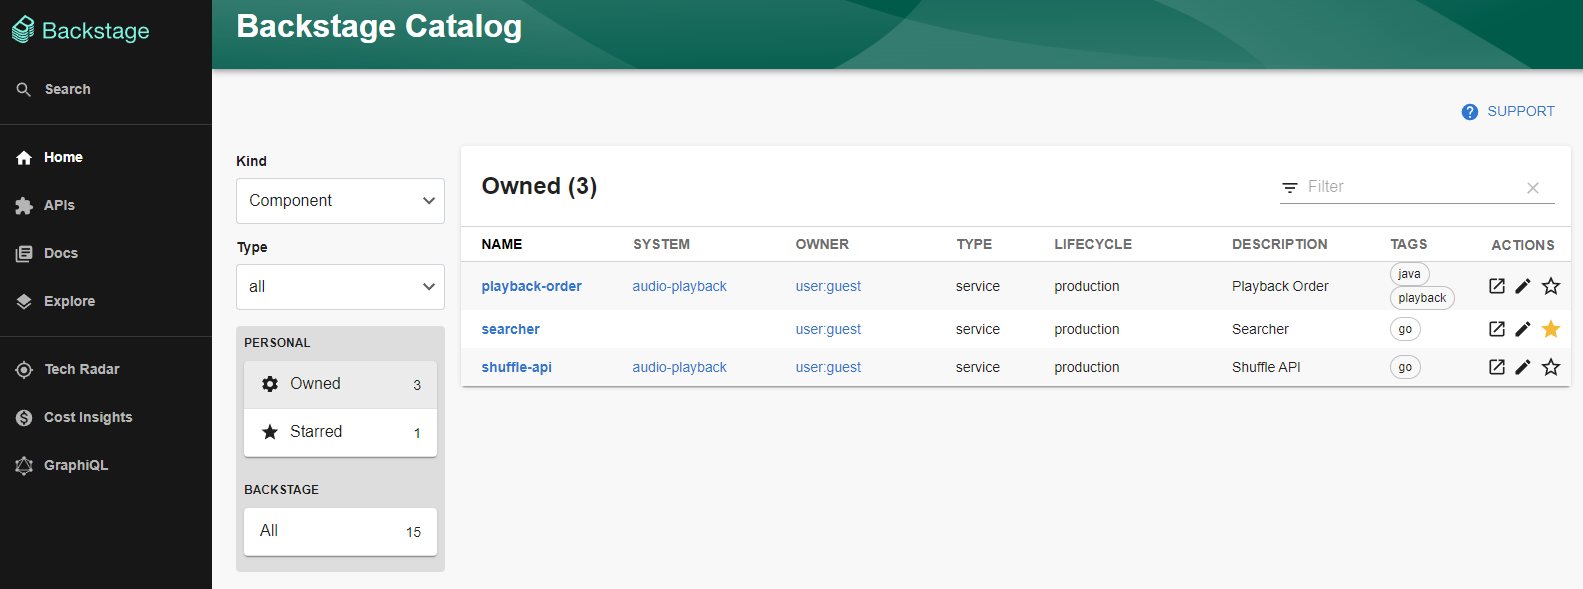
\includegraphics[width=\linewidth]{backstage_catalog}
        \caption{The Software Catalog from the Backstage Demo\parencite{backstagedemo}}
        \label{fig:catalog}
    \end{figure}
    The content of the catalog may be any combination of
    \begin{itemize}
        \item Teams with members
        \item Applications
        \item Infrastructure and platforms
        \item Most importantly, the relationships between those.
    \end{itemize}
    Data may be shown in a tabular fashion or as a relationship graph.
    The catalog allows a search over multiple entities.
    Usually, the user is already in his context.
    For example, the application where he' responsible are already loaded.
    An Engineer may bookmark its favourite items and its own resources are marked by ``owned``.
    In addition to the catalog with its tabular overview, there are detail views available as seen in figure \ref{fig:portaldetails}.
    \begin{figure}
        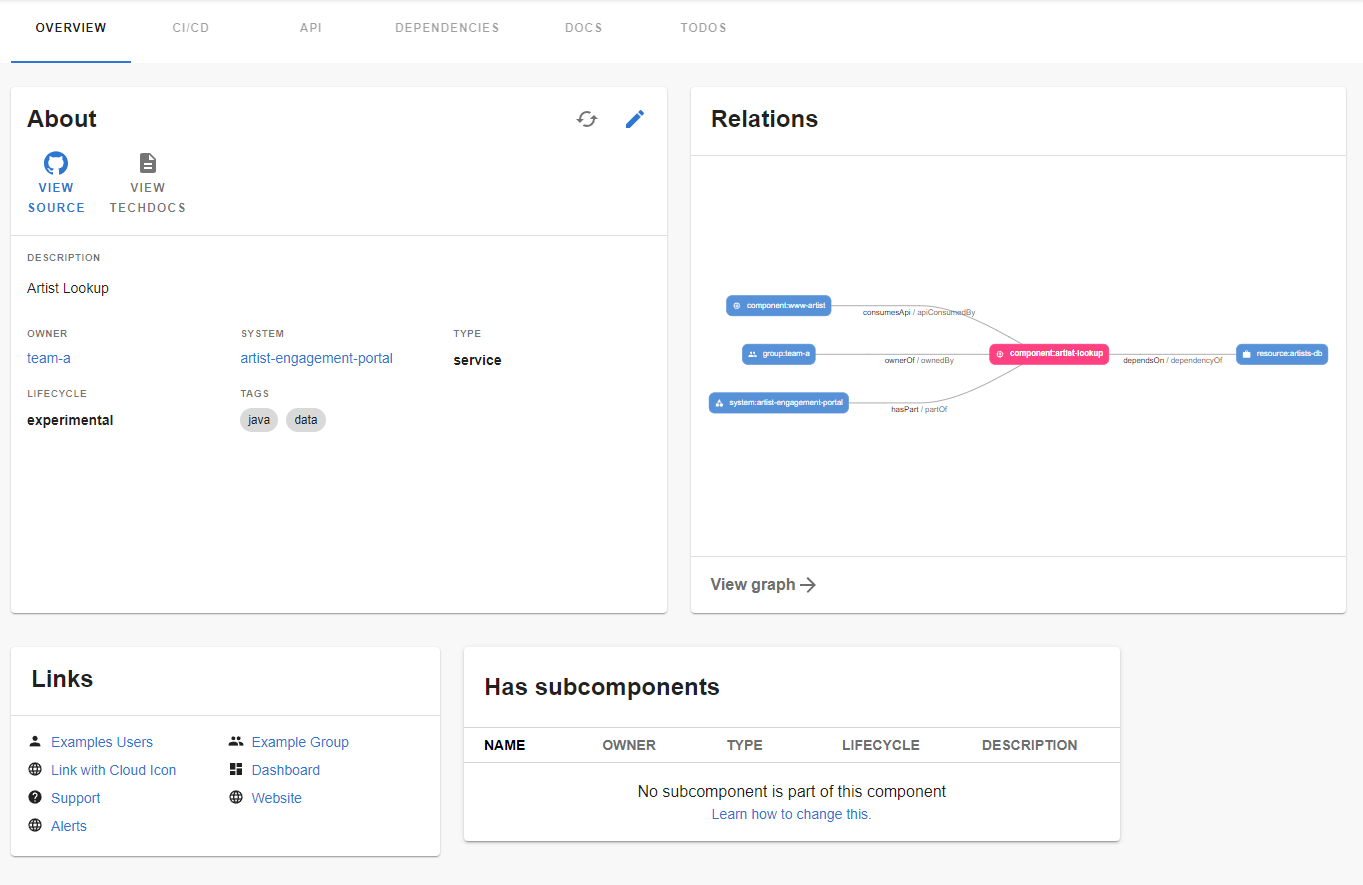
\includegraphics[width=\linewidth]{backstage_item_details}
        \caption{Details about an artifact}
        \label{fig:portaldetails}
    \end{figure}
    In the details view more attributes are shown for the chosen item from the overview.
    Depending on the kind of item, different attributes are shown.
    For an application, it may be its used resources, consumed and provided APIs and other subcomponents.
    For teams, the members are shown and their owned resources and the details how to contact the team.

    \subsubsection{Platform as a Product}
    \label{sssec:paap}
    In some implementations of an Internal Developer Portal, the catalog is not just a copy of an architecture database.
    In addition to the aforementioned applications, platforms, organizational data and resources, other products of the
    of the teams are represented.
    For example, platform teams may provide support and consulting for their platform or area of expertise and offer
    this service.
    Some teams use the Internal Developer Platform to showcase code or libraries solicit input or to create an
    inner-source community.\\
    In an expertise-sharing session between SBB and Booking.com, Booking.com reported\parencite{bookingcom} its Internal
    Developer Portal as a standalone product that is managed by a dedicated team.
    This team is also responsible for on-boarding other platform and application teams, convincing them of the
    value of an integrated Internal Developer Portal for the benefit of Booking.com.

    \subsubsection{Golden Path}
    \label{sssec:goldenpath}
    The term ``Golden Path`` was coined by Spotify\parencite{spotifygoldenpath} and is itself a reference to Frank
    Herbert`s Dune trilogy.
    The meaning of this term is, that there is only one viable path to do things right way and to succeed.
    A Golden Path in the context of an Internal Developer Portal is a ready-to-use template for getting a project
    started quickly.
    It can consist of software engineering artifacts and preconfigured infrastructure components and is usually very
    opinionated.
    Opinionated means that the context of the enterprise is already considered, such as internal regulations,
    architectural guidelines, the currently supported tech stack, and other internal specifications.
    For example, a golden path for a database is already built into the company's security infrastructure,
    logging is ensured, and some best practices for database configuration and modeling are implemented.\\
    Golden Paths are not necessarily product-specific;
    they can encompass a typical development stack used in the enterprise.
    For example a stack for a typical web application may consists of a frontend built with Javascript, a Java backend
    and an Oracle database, all integrated into a single build pipeline for CI/CD,    securely configured and with
    the enterprise look and feel already established.
    With such a template mechanism, new applications can be built faster and the same solutions are used for multiple
    applications.
    Additionally, the developers don't have to write tedious code to integrate each of these components with each other
    and can focus quickly on the business logic they have to implement.

    \subsubsection{Technical Documentation and Communication}
    \label{sssec:techdoc}
    Platforms that use an Internal Developer Portal may choose to migrate their user-facing documentation to the portal.
    The basis for this technical documentation can be a solution based on Markdown\parencite{backstagetechdocs}
    or a similar syntax.
    The advantage of this approach is that the documentation is treated like code and can be integrated into the same toolchain.
    For example, the documentation sits alongside the platform automation code, is peer reviewed, created
    and published in sync with the platform's update cycle.\\
    In the discussion mentioned in the chapter \ref{sssec:paap}, Booking.com talked about an integration in their Internal
    Developer Portal, where communication about lifecycle and changes to their platforms is also integrated into their portal.
    With this approach it is possible to inform DevOps engineers with targeted communication, especially combined with data about relationships
    between platforms, team resources and application as described in chapter \ref{sssec:disc}.
    This is especially important when communicating breaking changes, release notes or information about outages.

    \subsubsection{Making Expertise Visible}
    \label{sssec:expertise}
    Splunk\footnote{Splunk is a company specialised in creating software for log analysis and monitoring and it is known
    for its product with the same name}
    describes a use case, how to leverage an Internal Developer Portal to make expertise visible in their
    company\parencite{splunkidp} .
    One of the challenge is, that it is usually not transparent company wide which engineer has which speciality know-how.
    For example, one team integrated successfully a NoSql\footnote{NoSql databases are a broad class of databases which
    are not using the classic Structured Query Language (SQL). Examples are key/value stores, document oriented
    databases and others.  } database.
    This database is not part of a platform service but an integral part of a business applicaiton.
    The next team which would like to integrate the same technology faces the problem, that they have no internal
    expert for this technology and are not aware, that another team already did the legwork.
    The solution from Splunk is to enrich teams and users in the Internal Developer Portal with additional data about
    their knowledge and let other user give feedback how a team or user did support them, called a ``Bravo`` in their terminology.
    Thus, they create something like a social network inside their company for connecting people to solve problems or
    easing the way how to find people with specific skills or knowledge.

    \subsubsection{Extendability of the Platform}
    \label{sssec:extendability}
    As shown in chapter \ref{sssec:vendors}, there are multiple offerings of Internal Developer Portal and varying
    implementations.
    In case of the Software-as-a-Service offerings, the extendability consists of using plugins for well-known
    technologies or products and preparing and inserting the company's data for the catalogue feature.
    The self-hosted variants, such as Backstage and Clutch are more like a skeleton or a framework.
    For both products, there are pre-built binaries which are installable and runnable, but you can choose to build your
    own Internal Developer Portal and use these products as a starting point.
    Both support custom-made plugins on the front-end side which may use additional datasource outside the direct
    Internal Developer Portal.
    This approach is handy for decentralized organisational forms where each team have maximal autonomy about how they
    reach their goals, but would like to use and contribute to a centralized catalogue by adding data and functionality
    via plugins.
    The plugin architecture allows to leverage your Internal Developer Portal with the tooling landscape in a
    single and integrated user experience for DevOps Engineers.

    \subsubsection{FinOps}
    \label{sssec:finops}
    FinOps is a practice to enable DevOps Teams to make decisions about resource usage and creates transparency
    about the costs incurred by these decisions.
    The FinOps foundation defines\parencite{finopsdefinition} this practice as ``FinOps is an evolving cloud financial
    management discipline and cultural practice that enables organizations to get maximum business value by helping
    engineering, finance, technology and business teams to collaborate on data-driven spending decisions.``.
    An Internal Developer Portal may help with this practice by providing functionality for one of the basic disciplines
    of FinOps: ``Understanding Cloud Usage And Cost``.\\
    The Backstage.io Demo\parencite{backstagedemocost} shows one possible implementation.
    This capability enables a DevOps team to take responsibility also in the financial domain and creates transparency
    for the business what the true costs of their product is.


    \section{Situation at the SBB IT}
    \label{sec:sbbit}
    The IT department of the Swiss Federal Railways (SBB) consists of around 1300 specialists and is responsible for
    700 applications\parencite{sbbitkennzahlen}.
    The applications built and operated by this department are used for a wide range of use cases.
    For example, some applications are covering generic enterprise use cases such as human resource management, finance
    and controlling.
    Other software is specially built for mission-critical, day-to-day operations of the railway such as the Rail Control
    System (RCS)\parencite{sbbrcs} .\\
    An SBB IT application may be a purchased product, may be developed in-house or is a combination thereof which is
    sometimes called a ``customization``.\\
    Applications and products, built and operated by the SBB, are regulated by different standards and regulations of the
    swiss government or by industry initiatives.
    Examples are the EN 50128 standard by the European Committee for Electrotechnical Standardization (CENELEC)\parencite{cenelec},
    which governs among other things the development of safety-related software with different requirement levels.
    Another example is HCBöV\parencite{hcboev}, a swiss government regulation concerning cyber-security, risk management,
    business continuity management among others.\\
    In addition to the more business-oriented applications, there is a need for basic platforms, tools and services to help create
    and operate these applications.
    Examples for a foundational platform is a PaaS\footnote{A platform-as-a-service (PaaS) is a software which exposes
    resources such as compute or storage to applications. The team which is building an application is relieved from the
    burden of obtaining and provisioning resources on a hardware level. A well-known implementation of a PaaS is Kubernetes from the CNCF.}.
    This platform and other services are provided in the SBB by the so called DSRVs\footnote{
        A DSRV stands for Digital Service and is one or more teams with multiple services and platforms. A DSRV is built
        around a domain, eg. Monitoring, Cloud, Application Integration and others}.

    \subsection{Internal Developer Platform}
    \label{subsec:sbbplatform}
    The SBB IT has for most of the core components of an Internal Developer Platform, as laid out in chapter \ref{subsec:vpplatform},
    already solutions in place:
    \begin{itemize}
        \item Application Configuration Management - is centered around the practice of GitOps\parencite{hashicorpvault}
        \item Infrastructure Orchestration - for example, SBB uses OpenShift since 2015\parencite{rhsbbopenshift}
        \item Environment Management - provided by OpenShift and CI/CD Pipelines
        \item Deployment Management - is provided by CI/CD pipelines built on Tekton and ArgoCD\parencite{sbbtekton}
        \item Role-Based Access Control - built-in in most of the SBB IT platforms
    \end{itemize}
    In addition, there are several other tools and applications used for the day-to-day operations and development.
    Most notable are the following:
    \begin{itemize}
        \item Development and operation are dependent on a Wiki Software for documentation and communication.
        \item An Enterprise Architecture Database contains the information about used technologies, platforms and
        dependencies, modelled by IT architects
        \item An IT Service Management Platform contains the data concerning team contact information and support groups for applications
        \item A Configuration Management Database contains data about used assets, resources and relations to applications
    \end{itemize}
    Thus, it could be argued, that the foundation for an Internal Developer Platform is in place, but there are two
    critical pieces missing.
    First, most of the components mentioned are only partially integrated with each other.
    Examples for missing integration are different identifier for assets, unaligned authorization such as per-user vs.
    per-group models and manual data maintenance.
    Second, there is no central view to aggregate data contained in these applications and tools for the benefit of
    the DevOps engineers.

    \subsection{DevOps}
    \label{subsec:sbbdevops}
    In 2015, DevOps practices and a PaaS were introduced in SBB IT .
    The stated goal of these additions was to improve the increasing complexity in operations and the perceived slow
    speed in responding to change\parencite{sbbdevops}.\\
    Four years later, a reorganization brought a new operating model to the SBB IT based on agile principles, DevOps and
    SAFe, creating the role of BizDevOps engineer\parencite{sbbagile} .
    Most of the existing engineering roles, such as the Application Engineer, Operations Manager, Test Engineer or
    Requirements Engineer were transformed into this BizDevOps Engineer role.
    To bridge the gap between business and IT and break down silos, some business-facing roles have also been integrated into these
    cross-functional teams have been integrated and now have the title of a BizDevOps engineer.\\
    DevOps teams in SBB IT in 2023 are now the established standard.
    Despite this, they still work primarily with tools for development and operations from the predecessor organization.
    The tools themselves may be state-of-the-art in their areas, but they were not purchased or developed with
    end-to-end integration in mind.

    \subsection{Internal Developer Portal}
    \label{subsec:sbbportal}
    Most BizDevOps teams at SBB make do with additional structuring of their important information for daily work, to cope
    with the lack of a single and integrated portal.
    A common approach is to use the internal wiki software where each team maintains their relevant http link collection
    related to their project on one or more pages.
    In most cases, when someone joins a team, their first task is to familiarize themselves with this collection.
    Of course, these link collections become outdated and maintaining them also requires effort from a team.
    When entire teams are newly staffed, for example with models such as managed capacity or near-shore, it is even less
    easy for them to get all the information they need.\\
    While this discovery and knowledge sharing issue has not been fully resolved, there have been some efforts to create
    a self-service portal for ordering resources.
    The reason for this portal was that the platform teams were dissatisfied with the unstructured ordering of resources
    via email, phone, or other ad hoc methods.
    So a modular portal was built that allowed each team to integrate their ordering process.
    However, there was no single owner of the portal, and after the immediate pain point of each platform team was
    resolved, there was little effort to expand the functionality to include even more use cases.


    \section{Method}
    \label{sec:method}
    The method chosen to verify the observations about the state of the DevOps Experience and to evaluate the value proposition
    of an Internal Developer Portal, is to hold a survey.
    The survey is created with a customer journey based on different BizDevOps personas.
    The personas and the customer journey are based on a preliminary, internal work\parencite{sbbjobstobedone}.

    \subsection{Customer Journey}
    \label{subsec:cusjour}
    The customer journey is focused on the interaction of different personas with the existing Internal Developer Platform.
    The assumption is, that this interaction between the BizDevOps Engineers and the Internal Developer Platform has a big
    impact on the DevOps Experience.\\
    The personas of the customer journey are roles which are quite common in a BizDevOps team in the SBB IT.\\
    \textit{Peter Plattform} is working as a platform engineer and is interested what the platforms are offering for building
    an application.
    Peter orders a resource from a platform and is responsible over the full lifecycle until it this resource is not
    needed anymore.\\
    \textit{Diego Developer} is a software engineer and his duty is to work on features in the context of the application
    he' responsible for.
    He needs information about the current tech stack\footnote{A tech stack is short for technology stack.
    A technology stack is usually a selection of available componentes and framework such as databases, messaging, programming
    languages and other technologies necessary to build applications.} and he needs advice for the solution design of his application.
    Diego is also interested to get the releases of his application as fast as possible and with the highest quality
    into the production environment.\\
    \textit{Norbert Neuling} is the rookie in the team and started two days ago in this team.
    He needs first to install the necessary tooling to enable him to develop features.
    The next assignment for him for his learning journey is to create a sample application on OpenShift and integrate
    it with sample database provided.
    Additonally, Norbert needs some guidance about what the best practices are concerning the used technologies and platforms.\\
    \textit{Agnes Architekt} is working as an IT architect in the team.
    The product owner of the application she's responsible for, asked her to identify possibilities to lower the operational cost.
    She is also responsible for the enabler\footnote{An enabler is a work item which has no direct business value.
    For example a migration to a new version for a web framework or other technical necessities.} of the application.
    She has to create the necessary backlog items and communicates with the product owner, so that he can prioritize
    them and put them in one of the next product increments\footnote{SAFe terminology for a cycle of usually five two-week SCRUM Sprints of agile software development.}.
    For this work, she needs to know about the upgrade plans of the used services of the platforms her application is using.     \\
    \textit{Ida Incident} is working on an operational issue which is affecting the users of her application.
    She needs to know the technical topology of her application and the platforms which are used for operating this application.
    She needs to find the team which is responsible for a given platform and needs to know she can contact them.\\
    For more information about the customer journey, see figure \ref{fig:customerjourney}.

    \subsection{Quantitative Survey}
    \label{subsec:quansur}
    For a quantitative survey, a mix of questions were created based on the customer journey.
    Some relate to the value proposition of an Internal Developer Portal and others to other known or suspected issues
    related to the existing platform for internal developers.
    The survey is intentionally short, as longer surveys typically tend to show low response rates among BizDevOps engineers.
    The target audience for the survey is SBB's BizDevOps engineers around SBB IT's cloud platforms.
    One of the main sources of information for BizDevOps engineers is the CLEW\footnote{CLEW stands for Cloud, ESTA,
        itself an acronym of development stack and WZU, tool support} blog.
    This blog has a total of 780 subscribers.
    The survey itself was created using Microsoft Forms.
    The start date of the survey was 24.04.2023 and the end date was 08.08.2024.

    \subsubsection{Questions}
    \label{sssec:questions}
    Seventeen rating questions were created from the sixteen steps of the Customer Journey.
    The rating questions are documented in the appendix in the table \ref{tab:ratingquestionstable}.
    The relationship between the suggested value in chapter \ref{sec:vp} and the questions is as follows:
    \begin{itemize}
        \item question 1, 13, and 14 relate to discoverability and obtaining information in chapter \ref{sssec:disc}
        \item question 2 refers to making expertise visible from chapter \ref{sssec:expertise}
        \item questions 3 and 17 relate to technical documentation and communication, chapter \ref{sssec:techdoc}
        \item Question 10 refers to chapter \ref{sssec:goldenpath}, Golden Path.
        \item question 12 refers to FinOps, chapter \ref{sssec:finops}
    \end{itemize}
    Questions 4, 11, and 16 are not closely related to the concept of an Internal Developer Portal.
    However, these three questions are related to general capabilities of the existing platform for internal developers.\\
    Questions 5, 6, 7, 8, and 9 measure the maturity of the internal developer platform in terms of resource lifecycle.\\
    There are no direct questions about the Extendability \ref{sssec:extendability} chapter and Platform as a Product
    \ref{sssec:paap}.
    Extensibility is a non-functional requirement when selecting the specific solution for the Internal Developer Portal.
    This requirement is not the desire of a user of this portal and does not matter to them.\\
    Platform as a Product is a goal of SBB IT internal product management to make the work of BizDevOps
    team more visible and accessible and is not an intrinsic goal of an engineer.
    There is no question on this topic in the survey.\\
    Question 15 asks about support in the incident process and does not refer to an internal developer platform or an
    Internal Developer Portal. \\
    The survey and questions relate to DevOps experience and use of the platform, products, or services of the so-called CORE,
    which consists of multiple DSRVs, most with mission-critical platforms.
    It is not required that the respondent has used all services and platforms of the CORE.
    It is also scoped about usage of services and platforms in the last three months.\\
    The rating questions have choices from one to five stars and are all mandatory to complete.
    The meaning of the rating as defined as follows:
    \begin{itemize}
        \item One star - non-existent or unknown
        \item Two star - with room for improvement
        \item Three star - I can work with it, corresponds to what I expect
        \item Four star - above average
        \item Five star - super, that's what makes you
    \end{itemize}

    In addition, two other questions were asked, which are documented in table \ref{tab:oetable}.
    These questions are primarily for the internal needs of the product management of SBB IT platforms.
    They provide feedback on overall satisfaction and allow respondents to make additional points.
    One is a question with a that allows free text responses.
    The goal is to get additional input and to generate interview partners for a qualitative survey.
    This question is optional for the respondents.
    These interviews and the resulting findings are not part of this certificate thesis.\\
    The final question\{footnote{The engagement question was added based on input from the internal product management team}
    is an engagement question and is intended to measure the overall satisfaction of BizDevOps engineers related to the CORE platforms and services.
    % 2.3.2 Discoverability -> 1, 13, 14 (strong)
    %2.3.3 Platform as a Product n/a
    %2.3.4 Golden Path -> 10 (strong)
    %2.3.5 Technical Documentation, -> 3,17 -> ev. noch Extend! (strong)
    %2.3.6 Expertise -> 2, (strong)
    %2.3.7 Extendability
    %2.3.8 FinOps -> Frage 12. (strong)
    % n/a -> 4, 11, 16 (platform)
    % Lifecycle: -> 5, 6, 7, 8, 9 (weak)
    % monitoring, -> 15 (none)

    \subsubsection{Result of the Rating Questions}
    \label{sssec:rratque}
    After the two-week survey period, the response rate was 9.74\% with 76 respondents.
    Based on an industry standard 95\% confidence level\parencite{nistmean}, the margin of error for this survey for all
    Rating questions is 10\% for each.
    The raw results for the rating questions are included in table \ref{tab:rawratingquestionresultstable}.
    The calculated scores for the rating questions are included in table \ref{tab:ratingquestionresultstable}.
    Overall, the seventeen questions have an average score of 3.40, the average of negative responses (1.2) is 18.5\% of the
    respondents and the average of positive responses (4.5) is 51.3\%.
    Respondents with scores of 1 and 2 are counted among the detractors and respondents with 4 and 5 are counted as the promoters.
    The variance for the scoring questions ranges from 0.590 to 1.420.
    An aggregate result for the five value propositions with eight associated questions is documented in the table \ref{tab:aggregateidpresults}.
    \begin{table}[!htbp]
        \begin{center}
            \begin{tabularx}{\textwidth}{llllll}
                \toprule
                Topic           & Ids       & Average & Detractors & Promoters & Variance \\
                \midrule
                Discoverability & 1, 13, 14 & 3.11    & 24.4\%     & 35.1\%    & 0.826    \\
                Expertise       & 2         & 3.64    & 12.0\%     & 65.3\%    & 1.097    \\
                Documentation   & 3, 17     & 3.41    & 18.7\%     & 51.9\%    & 1.056    \\
                Golden Path     & 10        & 3.21    & 20.0\%     & 42.7\%    & 0.850    \\
                FinOps          & 12        & 2.62    & 45.3\%     & 21.3\%    & 1.420    \\
                \bottomrule
            \end{tabularx}
        \end{center}
        \caption{\label{tab:aggregateidpresults} Aggregated results for IDP related questions.}
    \end{table}
    In contrast, the aggregated results of questions on other topics are contained in the table \ref{tab:nonidpresults}.
    The results are grouped by resource lifecycle questions, generic questions about the internal developer platform
    and incident handling.

    \begin{table}[!htbp]
        \begin{center}
            \begin{tabularx}{\textwidth}{llllll}
                \toprule
                Topic     & Ids           & Average & Detractors & Promoters & Variance \\
                \midrule
                Lifecycle & 5, 6, 7, 8, 9 & 3.59    & 13.9\%     & 59.5\%    & 1.147    \\
                Platform  & 4, 11, 16     & 3.46    & 15.6\%     & 54.7\%    & 1.025    \\
                Incident  & 15            & 3.92    & 10.7\%     & 74.7\%    & 1.099    \\
                \bottomrule
            \end{tabularx}
        \end{center}
        \caption{\label{tab:nonidpresults} Aggregated results for non-IDP related questions.}
    \end{table}

    \subsubsection{Result of the Open Question}
    \label{sssec:ropque}
    32 of the 76 respondents answered the open question.
    Due to the sensitive nature of the answers regarding the technologies, teams and processes used, only some excerpts
    of the answers are reproduced in this chapter.
    The answers in full are documented in the internal wiki\cite{sbbdevopsexperience}.\\
    Six of the respondents mentioned the topic of Technical Documentation and Communication.
    One BizDevOps engineer would like to have ``Information und Dokumentation zentralisierter oder verknüpft.``.
    Another mentioned the decentralized communication about platform news: ``Man müsste eigentlich jemanden separat einstellen
    der all die Blogs etc. pp. im Auge behält. Es passiert immer wieder, dass irgendwo eine Information zwischen die
    Stühle fällt, weil es einfach aufgrund der Menge untergeht.``\\
    Four people mentioned the CI/CD pipelines.
    The older, but still supported, CI/CD pipeline was mentioned several times regarding issues. \\
    Three respondents had some suggestions for additional tools in the development tools installer and additional
    feedback for it.
    This topic was covered in question 4.
    One respondent was very pleases and said about the setup process for development tools: ``In 15 Minuten
    Entwicklungsumgebung aufsetzen und los coden ist schon geil! :-)``\\
    Three respondents simply stated their gratitude and thanked the various service and platform teams of the CORE for
    their effort.
    For example, one respondent simply wrote ``danke, von Herz``.\\
    Two respondents mentioned the topic of financial transparency, covered by the question 12.
    One quote about this topic by an BizDevOps engineer was: ``Kosten sind sehr schwierig zu verstehen und nachvollziehen auf die Rechnung. Reporting
    sollte unbedingt verbessert sein, man weiss nicht wo man könnte optimieren (zu beispiel welche anteil von kosten für
    xyz kommt von storage? von anzahle objekte? usw.)``\\
    There were also two suggestions about missing infrastructure as code capabilities.\\
    Two feedback concerned the current vision and its wording of the so called CORE DSRVs.\\
    Two questioned a perceived lack of consultancy and unified support.\\
    And finally, there were two critical votes about the modernization effort of the SBB IT which is known as the
    ''Gandalf Plan'' and the perceived primacy of technology enabler over features for the business.\\
    Six feedbacks each concerned different other topics which will not be discussed in more detail.
    % techdoc + Benach: IIIIII
    % CI/CD kritik: IIII
    % Discovery: IIII
    % Enhancement local installation: III
    % thanks: III
    % finOps: II
    % infrastructure-as-code missing: II
    % critic of vision: II
    % missing consultancy / unified support: II
    % gandalf kritik: II
    % multiple tools for the same job: I
    % Availability of toolchainL: I
    % non-informatiker: I
    % missing review/freigabeprozess: I
    % missing resource lifecycle for delete, upgrade: I
    % missing devsecops: I

    \subsubsection{Result of the Engagement Question}
    \label{sssec:rengque}
    The average result of the engagement question was 7.70 with a variance of 2.080.
    The distribution can be seen in figure \ref{fig:engque}.
    \begin{figure}
        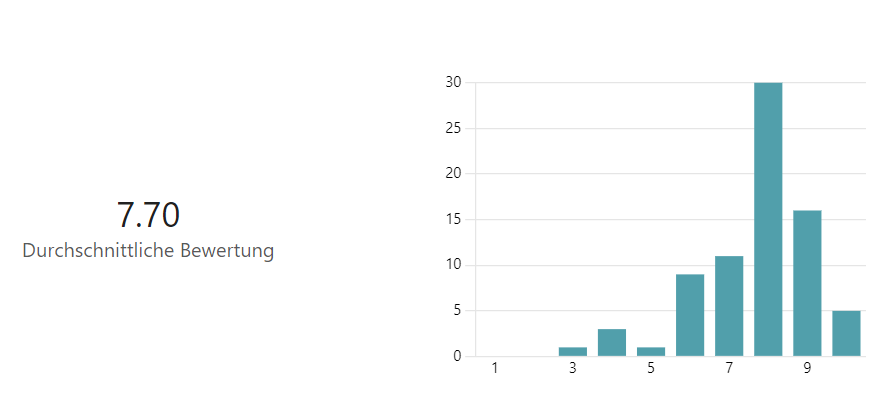
\includegraphics[width=\linewidth]{engagement.PNG}
        \caption{Results of the Engagement Question}
        \label{fig:engque}
    \end{figure}
    The result of the engagement question is not relevant for evaluating the value proposition.
    It is valuable to gauge the overall net promoter score\parencite{nps} of the CORE platforms and services.
    \begin{itemize}
        \item Values between 1 to 6 are considered detractors. Fourteen responses fell into this category.
        \item Values between 7 and 8 are considered passives, forty-one responses fell into this range.
        \item Values between 9 and 10 are considered as promoters. Twenty-one responses fell into this category.
    \end{itemize}
    With the NPS method applied, there are 18.42\% detractors and 27.63\% promoters which amounts to a net NPS Score of
    9.21\%.


    \section{Conclusion}
    \label{sec:conclusion}
    Based on the data from the evaluation questions in chapter \ref{sssec:rratque}, the value propositions of
    Discoverability and Obatining Information, Golden Path, and FinOps are below the average for all questions (3.40)
    and outside the margin of error (10\%).
    The average of the Documentation and Communication theme is 3.41, almost on par with the overall average.
    The topic Making Expertise Visible has an average score of 3.64, which is above the overall average.
    Topics not directly related to the internal developer portal are at or above the overall average.
    General platform topics have an average score of 3.46, which is near the overall average.
    Lifecycle of Resources has an average score of 3.59 and the Incident Support topic has an average of 3.92.\\
    Summary of Data;
    \begin{itemize}
        \item Three of the five, in the survey tested, value propositions of an Internal Developer Portal are below the overall average and outside the error margin.
        \item Two of the three other topics are above and one is near the overall average of the survey.
        \item Fifteen answers for the open-ended questions contain issues related to the value propositions of an Internal Developer Portal
    \end{itemize}
    Thus, there is an argument, that an Internal Developer Portal could be of value for the BizDevOps engineers if the following
    criteria are met:
    \begin{itemize}
        \item The solution must have have some kind of a FinOps capability.
        \item The solution must improve the discoverability of services, teams, resources and platforms.
        \item The solution must have the capability to publish Golden Path
    \end{itemize}
    There could be additional benefit for the BizDevOps engineers, if the solution also has the capability to aid with
    Documentation functionality and makes it more accessible.
    There seems no current need to use an Internal Developer Portal for making Expertise more visible.

    \subsection{Recommendations for Action}
    \label{subsec:arec}
    The recommendations for action are for SBB IT with the current status in May 2023 regarding the Internal Developer Platform.

    \subsubsection{Prioritize Relationships}
    From the evaluation questions to the answers to open questions to additional direct feedback outside of the survey,
    there is repeated criticism that there is no capability to have an integrated view of applications, teams, platforms
    used, and resources.
    There is currently no platform of this kind and could be the unique selling point of this internal developer platform.

    \subsubsection{Target BizDevOps Engineer}
    There is value in targeting the needs of the BizDevOps Engineers.
    They are lacking a coherent view for operating applications and improvements should be felt immediately by falling
    KPIs like MTTR\footnote{MTTR stands for mean time to repair. Its the measured time between a failure of a system
    until it is fixed again and in working order.} or an improved future net promoter score, the current value is 9.21\%
    as calculated in chapter \ref{sssec:rengque}.\\
    Refrain initially from targeting other roles such as management, architects, security or non BizDevOps teams with
    an Internal Developer Portal to not dilute the focus of the Internal Developer Portal and maximizing the impact on
    the work of the BizDevOps engineers.
    If necessary, try to onboard such additional users and use cases later on.

    \subsubsection{Don't Try to Replace Existing Tooling}
    It is tempting to use an Internal Developer Portal as an opportunity to simplify and consolidate the existing tooling
    landscape, for example the components of the Internal Developer Platform.
    Remember, the Internal Developer Portal is only the frontend and makes the Internal Developer Platform accessible
    as seen in chapter \ref{subsec:vpplatform}.
    Most of the presented vendors and products in chapter \ref{sssec:vendors} have the capability and the frameworks
    necessary to achieve this separation of concern.

    \subsubsection{Prioritize Missing Capabilities}
    Try to prioritize missing capabilities such as the mentioned FinOps instead of building again well understand and already
    implemented features such as ordering a resource.

    \subsubsection{Focus on Runtime Data}
    There is no need to build again an enterprise application database.
    IT Architects are using the established database for modelling their solutions and thus it may not reflect the current
    state of an application.
    Focus instead on the runtime data.
    For example, use data such as which application is deployed on a platform, telemetry data of applications or platforms or
    configured resources if GitOps\footnote{
        GitOps is a practice where resource definitions are stored in a source code version system. If any change
        happens in this definitions, the values are synced to a runtime, for example to a Kubernetes cluster.} is used.

    \pagebreak
    % max 15 - 20 pages end here


    \section{List of Sources}
    \label{sec:bibliograhpy}
    \printbibliography[heading=none]


    \section{Appendix}
    \label{sec:appendix}

    \subsection{Customer Journey Map}
    \label{subsec:cusjourmap}
    \begin{landscape}
        \begin{figure}[h]
            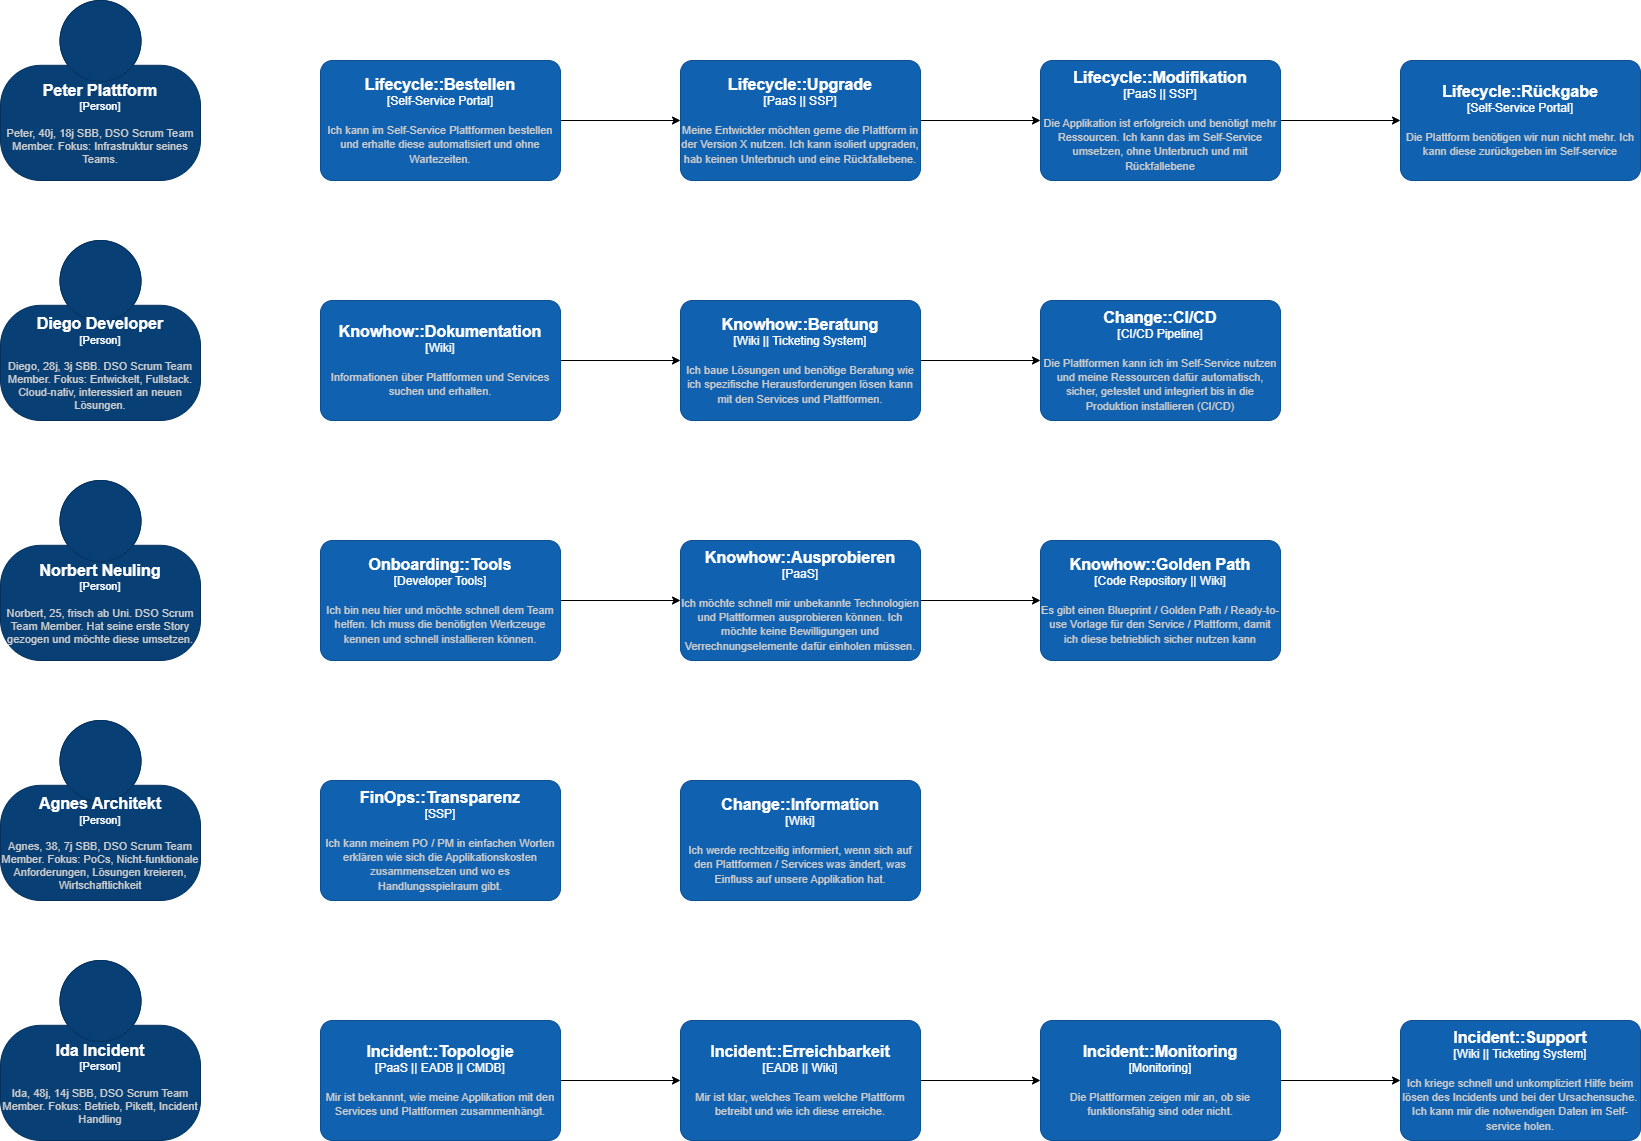
\includegraphics[origin=c,width=0.9\linewidth]{customer-journey.png}
            \caption{Customer Journey Map}
            \label{fig:customerjourney}
        \end{figure}
    \end{landscape}

    \subsection{Survey}
    \label{subsec:survey}

    \subsection{Rating Questions}
    \label{subsec:rating}
    \begin{table}[!htbp]
        \begin{center}
            \begin{tabularx}{\textwidth}{lX}
                \toprule
                Id & Question                                                                                                                                                                              \\
                \midrule
                1  & Auffindbarkeit von Informationen über die Plattformen und Services. Zb. Confluence, Ardoq, Intranet...                                                                                \\
                2  & Ich kriege schnell und unkompliziert Beratung bei der Konzipierung von Applikationen, zb. für Engineering oder Development.                                                           \\
                3  & Qualität der Dokumentation der Plattformen und Services (Sowohl Umfang, Aktualität und Inhalt).                                                                                       \\
                4  & Onboarding, bis ich meine Werkzeuge für Dev oder Ops lokal installiert habe.                                                                                                          \\
                5  & Lifecycle von Infrastruktur im Selfservice, hier; ich kann Services und Plattformen schnell und unkompliziert ausprobieren.                                                           \\
                6  & Lifecycle von Infrastruktur im Self-Service, hier Bestellen von Plattformen                                                                                                           \\
                7  & Lifecycle von Infrastruktur im Self-Service, hier, Upgrade von Plattformen / deiner Applikation auf den Plattformen                                                                   \\
                8  & Lifecycle von Infrastruktur im Self-Service, hier Modifikation von Plattformen oder Applikationen.                                                                                    \\
                9  & Lifecycle von Infrastruktur im Self-Service, hier Run-Down oder Rückgabe von Plattformen                                                                                              \\
                10 & Es gibt einen Blueprint / Golden Path / Vorlage, die mir zeigt, wie ich eine Plattform verwenden kann.                                                                                \\
                11 & Die Plattformen erlauben mir, meine Ressourcen automatisiert zu bauen und zu deployen (CI/CD)                                                                                         \\
                12 & Ich kann meinem PO die Kosten unserer genutzten Services und Plattformen nachvollziehbar erklären.                                                                                    \\
                13 & Ich verstehe, wie meine Applikation mit den Plattformen zusammenhängt bei Incidents                                                                                                   \\
                14 & Welches DSRV Team für welche Plattform verantwortlich ist, ist mir klar.                                                                                                              \\
                15 & Ich kriege schnell und unkompliziert Hilfe im Incident Fall.                                                                                                                          \\
                16 & Die Plattformen zeigen mir an, ob sie funktionsfähig sind oder nicht. (zb. Monitoring, Chat, ...).                                                                                    \\
                17 & Ich, bzw. mein Team, werden rechtzeitig und mit genug Details informiert, wenn sich auf den Plattformen etwas ändert, was Auswirkungen auf die von uns verantwortete Applikation hat. \\
                \bottomrule
            \end{tabularx}
        \end{center}
        \caption{\label{tab:ratingquestionstable} Rating questions used in the survey.}
    \end{table}

    \subsection{Open and Engagement Questions}
    \label{subsec:openandengagement}
    \begin{table}[!htbp]
        \begin{center}
            \begin{tabularx}{\textwidth}{lX}
                \toprule
                Id & Question                                                                                                                                                                                                                                                                      \\
                \midrule
                18 & Was du uns sonst noch mit auf den Weg geben willst für die ``geilste DevOps Experience``, die du erleben möchtest. Falls du bereit bist, in einem kleinen Interview noch mehr Auskünfte zu erteilen und Nachfragen zu beantworten, gib uns doch hier auch deine Kontaktdaten. \\
                19 & Auf einer Skala von 1 \- 10, würdest du CORE (die genannten DSRVs und deren Plattformen) deinen Freunden und Arbeitskollegen weiterempfehlen?                                                                                                                                 \\
                \bottomrule
            \end{tabularx}
        \end{center}
        \caption{\label{tab:oetable} Open and engagement questions used in the survey.}
    \end{table}
    \FloatBarrier

    \subsection{Rating Questions Results}
    \label{subsec:ratingresults}
    \begin{table}[!htbp]
        \begin{center}
            \begin{tabularx}{\textwidth}{llllll}
                \toprule
                Id & One Star & Two Star & Three Star & Four Star & Five Star \\
                \midrule
                1  & 3        & 12       & 40         & 21        & 0         \\
                2  & 5        & 4        & 18         & 35        & 14        \\
                3  & 1        & 13       & 30         & 30        & 2         \\
                4  & 8        & 6        & 23         & 28        & 11        \\
                5  & 6        & 7        & 20         & 25        & 18        \\
                6  & 1        & 5        & 17         & 29        & 24        \\
                7  & 5        & 4        & 20         & 35        & 12        \\
                8  & 5        & 3        & 25         & 31        & 12        \\
                9  & 8        & 8        & 23         & 26        & 11        \\
                10 & 4        & 11       & 29         & 29        & 3         \\
                11 & 2        & 4        & 20         & 34        & 16        \\
                12 & 17       & 17       & 26         & 10        & 6         \\
                13 & 1        & 11       & 31         & 24        & 9         \\
                14 & 6        & 22       & 23         & 22        & 3         \\
                15 & 3        & 5        & 12         & 31        & 25        \\
                16 & 4        & 11       & 27         & 30        & 4         \\
                17 & 3        & 11       & 18         & 31        & 13        \\
                \bottomrule
            \end{tabularx}
        \end{center}
        \caption{\label{tab:rawratingquestionresultstable} Raw results for the rating questions.}
    \end{table}

    \begin{table}[!htbp]
        \begin{center}
            \begin{tabularx}{\textwidth}{lllll}
                \toprule
                Id & Average & Detractors & Promoters & Variance \\
                \midrule
                1  & 3.04    & 20.0\%     & 28.0\%    & 0.590    \\
                2  & 3.64    & 12.0\%     & 65.3\%    & 1.097    \\
                3  & 3.25    & 18.7\%     & 42.7\%    & 0.661    \\
                4  & 3.37    & 18.7\%     & 52.0\%    & 1.312    \\
                5  & 3.55    & 17.3\%     & 57.3\%    & 1.379    \\
                6  & 3.92    & 8.0\%      & 70.7\%    & 0.915    \\
                7  & 3.59    & 10.7\%     & 62.7\%    & 1.057    \\
                8  & 3.55    & 21.3\%     & 57.3\%    & 1.037    \\
                9  & 3.32    & 20.0\%     & 49.3\%    & 1.348    \\
                10 & 3.21    & 20.0\%     & 42.7\%    & 0.850    \\
                11 & 3.76    & 8.0\%      & 66.7\%    & 0.865    \\
                12 & 2.62    & 45.3\%     & 21.3\%    & 1.420    \\
                13 & 3.38    & 16.0\%     & 44.0\%    & 0.841    \\
                14 & 2.92    & 37.3\%     & 33.3\%    & 1.046    \\
                15 & 3.92    & 10.7\%     & 74.7\%    & 1.099    \\
                16 & 3.25    & 20.0\%     & 45.3\%    & 0.898    \\
                17 & 3.53    & 18.7\%     & 58.7\%    & 1.118    \\
                \bottomrule
            \end{tabularx}
        \end{center}
        \caption{\label{tab:ratingquestionresultstable} Calculated results for the rating questions.}
    \end{table}

\end{document}